\documentclass[10pt]{article}
\usepackage{tikz}
\usetikzlibrary{shapes.misc}
\usepackage[margin=0cm]{geometry}
\pagestyle{empty}
\tikzstyle{every node}=[cross out, draw, red]

\begin{document}

\vspace*{\fill}
\begin{center}
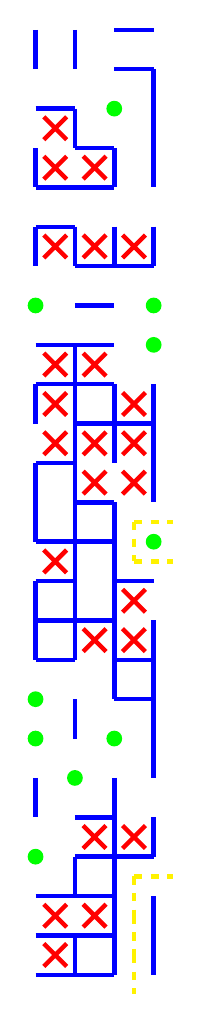
\begin{tikzpicture}[x=0.5cm, y=-0.5cm, ultra thick, blue]
% Walls
    \draw (0, 0) -- (0, 1);
    \draw (1, 0) -- (1, 1);
    \draw (2, 0) -- (3, 0);
    \draw (2, 1) -- (3, 1);
    \draw (3, 1) -- (3, 2);
    \draw (3, 2) -- (3, 3);
    \draw (3, 3) -- (3, 4);
    \draw (2, 3) -- (2, 4);
    \draw (0, 3) -- (0, 4);
    \draw (1, 3) -- (2, 3);
    \draw (1, 2) -- (1, 3);
    \draw (0, 2) -- (1, 2);
    \draw (1, 4) -- (2, 4);
    \draw (0, 4) -- (1, 4);
    \draw (1, 6) -- (2, 6);
    \draw (2, 6) -- (3, 6);
    \draw (0, 5) -- (1, 5);
    \draw (0, 5) -- (0, 6);
    \draw (1, 5) -- (1, 6);
    \draw (2, 5) -- (2, 6);
    \draw (3, 5) -- (3, 6);
    \draw (1, 7) -- (2, 7);
    \draw (1, 17) -- (1, 18);
    \draw (1, 12) -- (2, 12);
    \draw (1, 12) -- (1, 13);
    \draw (1, 9) -- (2, 9);
    \draw (1, 9) -- (1, 10);
    \draw (0, 8) -- (1, 8);
    \draw (2, 16) -- (3, 16);
    \draw (2, 16) -- (2, 17);
    \draw (1, 15) -- (2, 15);
    \draw (1, 15) -- (1, 16);
    \draw (3, 17) -- (3, 18);
    \draw (0, 14) -- (1, 14);
    \draw (0, 14) -- (0, 15);
    \draw (3, 10) -- (3, 11);
    \draw (2, 12) -- (2, 13);
    \draw (0, 9) -- (1, 9);
    \draw (0, 9) -- (0, 10);
    \draw (1, 8) -- (2, 8);
    \draw (1, 8) -- (1, 9);
    \draw (3, 16) -- (3, 17);
    \draw (0, 15) -- (1, 15);
    \draw (0, 15) -- (0, 16);
    \draw (2, 17) -- (3, 17);
    \draw (1, 14) -- (1, 15);
    \draw (1, 11) -- (1, 12);
    \draw (2, 13) -- (2, 14);
    \draw (3, 15) -- (3, 16);
    \draw (3, 9) -- (3, 10);
    \draw (0, 11) -- (1, 11);
    \draw (0, 11) -- (0, 12);
    \draw (0, 16) -- (1, 16);
    \draw (1, 10) -- (2, 10);
    \draw (1, 10) -- (1, 11);
    \draw (2, 14) -- (3, 14);
    \draw (2, 14) -- (2, 15);
    \draw (1, 13) -- (2, 13);
    \draw (1, 13) -- (1, 14);
    \draw (3, 18) -- (3, 19);
    \draw (2, 15) -- (2, 16);
    \draw (0, 12) -- (0, 13);
    \draw (2, 9) -- (2, 10);
    \draw (3, 11) -- (3, 12);
    \draw (0, 13) -- (1, 13);
    \draw (2, 10) -- (3, 10);
    \draw (2, 10) -- (2, 11);
    \draw (0, 19) -- (0, 20);
    \draw (3, 22) -- (3, 23);
    \draw (3, 23) -- (3, 24);
    \draw (3, 20) -- (3, 21);
    \draw (2, 21) -- (3, 21);
    \draw (2, 21) -- (2, 22);
    \draw (1, 20) -- (2, 20);
    \draw (2, 19) -- (2, 20);
    \draw (1, 23) -- (2, 23);
    \draw (1, 23) -- (1, 24);
    \draw (0, 24) -- (1, 24);
    \draw (0, 22) -- (1, 22);
    \draw (2, 22) -- (2, 23);
    \draw (1, 21) -- (2, 21);
    \draw (1, 21) -- (1, 22);
    \draw (2, 20) -- (2, 21);
    \draw (2, 23) -- (2, 24);
    \draw (0, 23) -- (1, 23);
    \draw (1, 24) -- (2, 24);
    \draw (1, 22) -- (2, 22);
% Pillars
    \fill[green] (2, 2) circle(0.2);
    \fill[green] (0, 7) circle(0.2);
    \fill[green] (3, 7) circle(0.2);
    \fill[green] (3, 8) circle(0.2);
    \fill[green] (3, 13) circle(0.2);
    \fill[green] (0, 17) circle(0.2);
    \fill[green] (0, 18) circle(0.2);
    \fill[green] (2, 18) circle(0.2);
    \fill[green] (1, 19) circle(0.2);
    \fill[green] (0, 21) circle(0.2);
% Inner points in accessible cul-de-sacs
    \node at (0.5, 2.5) {};
    \node at (0.5, 3.5) {};
    \node at (1.5, 3.5) {};
    \node at (0.5, 5.5) {};
    \node at (1.5, 5.5) {};
    \node at (2.5, 5.5) {};
    \node at (0.5, 8.5) {};
    \node at (1.5, 8.5) {};
    \node at (0.5, 9.5) {};
    \node at (0.5, 10.5) {};
    \node at (2.5, 9.5) {};
    \node at (1.5, 10.5) {};
    \node at (2.5, 10.5) {};
    \node at (1.5, 11.5) {};
    \node at (2.5, 11.5) {};
    \node at (0.5, 13.5) {};
    \node at (1.5, 15.5) {};
    \node at (2.5, 14.5) {};
    \node at (2.5, 15.5) {};
    \node at (1.5, 20.5) {};
    \node at (2.5, 20.5) {};
    \node at (0.5, 22.5) {};
    \node at (1.5, 22.5) {};
    \node at (0.5, 23.5) {};
% Entry-exit paths without intersections
    \draw[dashed, yellow] (2.5, 12.5) -- (3.5, 12.5);
    \draw[dashed, yellow] (2.5, 12.5) -- (2.5, 13.5);
    \draw[dashed, yellow] (2.5, 13.5) -- (3.5, 13.5);
    \draw[dashed, yellow] (2.5, 21.5) -- (3.5, 21.5);
    \draw[dashed, yellow] (2.5, 21.5) -- (2.5, 22.5);
    \draw[dashed, yellow] (2.5, 22.5) -- (2.5, 23.5);
    \draw[dashed, yellow] (2.5, 23.5) -- (2.5, 24.5);
\end{tikzpicture}
\end{center}
\vspace*{\fill}

\end{document}